\section{Experiments}
\label{sec:exp}

To measure Legion's ability to distribute work across a distributed machine, 
two real-world benchmarks were run on a cluster under a
variety of configurations.  The cluster consists of four nodes connected by a
40~Gb/s Infiniband fabric.  Each node is powered by 2 Intel Xeon X5680 CPUs,
each with 6 cores, and 2 NVIDIA Tesla C2070 GPUs.  The cluster is running Linux
with GASNet using the {\tt ibv} conduit to interface directly with the standard
OFED software stack for low-latency access to the Infiniband hardware.

%%%%%%%%%%%%%%%%%%%%%%%%%%%%%%%%%%%%%%%%%%%%%%%%%%%%%%%%%%%%%%%%%%%%%%%%%

\subsection{Circuit Simulator}

The circuit simulator benchmark was designed to be representative of the
general class of finite-element simulations on irregular grids.  It relies
on many iterations using small stencils (e.g. just the neighboring nodes) to
propagate changes through the system.  Each iteration requires communication
between neighboring nodes.  Careful partitioning of the system can minimize
the amount of information that must be exchanged, but the irregularity of the
underlying graph mandates similar irregularity in the sharing pattern.

The structure of the circuit simulator was presented in Section~\ref{sec:ex}.
Our implementation uses CUDA to perform the computations on the GPU, and Legion
automatically handles the movement of data between the GPUs' memories and the
system memory when communication is necessary.  By utilizing an  
application-specific mapper, our implementation is able to keep much of
the data permanently resident in a given GPU for the entirety of the simulation.
Figure ~\ref{sfig:results1:perf} shows the relative speedup as the simulation is
spread over multiple nodes in the cluster.  We demonstrate strong scaling by
keeping the size of the circuit fixed as node count increases.
Adding a second node to the simulation
speeds it up by 86\%, and with four nodes, the simulation is sped up by a total
of 241\% (i.e. a factor of 3.41x).  When enabling the use of both GPUs in each
node (a decision that requires no changes to the application), we achieve
a speedup of 5.90x when using all eight GPUs.

The dip in the performance graph for the 6 GPU case is an artifact of the
application code's decision to partition the circuit into 8 pieces.  The
current runtime interface does not allow the application to make queries
regarding the machine configuration, so it is not able to adapt to
configurations that differ from the initial design target.  The Legion runtime
will always guarantee correct execution, but performance can suffer if the
tasks provided by the application do not divide evenly over the machine.

Table~\ref{sfig:results1:timers} breaks down the execution time by where it was
spent.  The times are summed over all threads, so the aggregate execution time
will always exceed the elapsed wall clock time.  The time spent in the 
application code is nearly constant in all configurations, but the time spent
copying data jumps as soon as the simulation is spread across multiple nodes.
This is not unexpected, and while the the overhead is responsible for the
less-than-linear performance scaling, the slow growth in the absolute overhead
(after the initial jump) suggests that larger clusters would enjoy additional
speedup, even without increasing the size of the problem being tackled.

\pgfplotsset{every axis legend/.append style={
  font=\tiny,
  at={(0.02,0.98)},
  anchor=north west},
  cycle list={{black, mark=x}, {black, mark=+},
              {black, mark=o}, {black, mark=diamond},
              {black, mark=triangle}, {black, mark=star}}}

\begin{figure}
  \centering
  \subfigure[Performance Scaling]{
    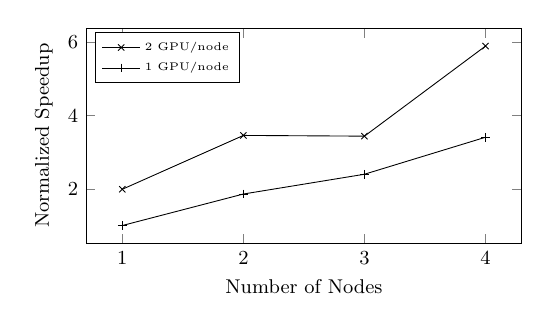
\begin{tikzpicture}[scale=0.8]
      \begin{axis}[xlabel=Number of Nodes,ylabel=Normalized Speedup,height=5cm,width=8.5cm,xtick={1,2,3,4},font=\small]
        \addplot coordinates {
% num gpus = 2
  (1, 1.99)
  (2, 3.46)
  (3, 3.44)
  (4, 5.90)
        };
        \addplot coordinates {
% num gpus = 1
  (1, 1.00)
  (2, 1.86)
  (3, 2.40)
  (4, 3.41)
        };
      \legend{2 GPU/node,1 GPU/node}
      \end{axis}
    \end{tikzpicture}
    \label{sfig:results1:perf}
  }

  \subtable[Execution Time Breakdown (all times in s)]{
    \scalebox{0.8}{
   \tiny
    \begin{tabular}{c@{\hspace{2pt}}cD{.}{.}{3}D{.}{.}{3}@{\hspace{2pt}}D{.}{.}{3}@{\hspace{2pt}}D{.}{.}{3}@{\hspace{2pt}}D{.}{.}{3}@{\hspace{2pt}}D{.}{.}{3}@{\hspace{2pt}}D{.}{.}{3}}
\toprule
GPUs/ & \# \\
node & nodes & \multicolumn{1}{c}{Wall Clock} & \multicolumn{1}{c}{Application} & \multicolumn{1}{c}{Copies} & \multicolumn{1}{c}{High-level} & \multicolumn{1}{c}{Low-level} & \multicolumn{1}{c}{Mapper} & \multicolumn{1}{c}{System} \\
\midrule
\multirow{4}{*}{$1$} & $1$ & 106.892 & 105.387 & 1.578 & 0.003 & 21.624 & 0 & 0\\
 & $2$ & 57.388 & 105.407 & 10.348 & 0.003 & 15.177 & 0 & 0.001\\
 & $3$ & 44.552 & 105.41 & 11.935 & 0.003 & 11.695 & 0 & 0.002\\
 & $4$ & 31.368 & 105.42 & 12.875 & 0.004 & 8.419 & 0 & 0.003\\
\midrule
\multirow{4}{*}{$2$} & $1$ & 53.787 & 105.397 & 1.857 & 0.004 & 10.953 & 0 & 0\\
 & $2$ & 30.923 & 105.415 & 10.716 & 0.004 & 7.937 & 0 & 0.002\\
 & $3$ & 31.037 & 105.414 & 12.558 & 0.004 & 7.996 & 0 & 0.001\\
 & $4$ & 18.103 & 105.42 & 13.747 & 0.004 & 4.638 & 0 & 0.003\\
\bottomrule \\
    \end{tabular}
}
    \label{sfig:results1:timers}
  }
  \caption{Circuit Simulator Results}
\end{figure}

\pgfplotsset{every axis legend/.append style={
  font=\tiny,
  at={(0.02,0.98)},
  anchor=north west}}

%%%%%%%%%%%%%%%%%%%%%%%%%%%%%%%%%%%%%%%%%%%%%%%%%%%%%%%%%%%%%%%%%%%%%%%%%

\subsection{Fluid}

To show that Legion remains efficient for regular partitioning cases as well,
we have implemented a particle simulation benchmark based on the
{\tt fluidanimate} benchmark from the PARSEC \cite{bienia11benchmarking} suite.
Our simulation uses a cyclic 2D grid of cells instead of PARSEC's 3D grid with
boundaries, but the computations being performed are preserved.
Although the 
simulation is moving and colliding individual particles, those particles
are placed in cells that make up a regular grid.  The grid is
divided into blocks to be processed by individual threads, with only the
particles in the edge cells being of interest to other threads.  The PARSEC
implementation uses fine-grained locking and the assumption of cache
coherence to access neighboring particles, but neither of these are conducive
to performance scaling across a cluster.  Our fluid benchmark replaces these
accesses with rings of
explicit edge, or \emph{ghost}, cells that are exchanged between adjacent
blocks several times per iteration.  The capturing of these inter-block
interactions through edge cells and the partitioning of those cells into
subregions provides the runtime the ability to schedule data movement in
advance and perform a more precise enforcement of the ordering
constraints necessary for correctness (e.g.
requiring a task to wait only for the subset of tasks in the previous pass 
that computed one of the ghost cells being read by this task).

Figure~\ref{sfig:results2:perf} shows the throughput of the fluid benchmark when
run on various subsets of the CPUs and nodes in the cluster.  Performance is
normalized with respect to the serial execution case.  As in the circuit
simulation case, the same size problem is used for all runs, and we see 
speedups of up to 10.14x when using the entire cluster (a total of 48 CPUs).
The execution time breakdown in Table~\ref{sfig:results2:timers} shows some
differences in scaling behavior compared to the circuit simulation.  The time
spent performing copies is much smaller on absolute scale, but shows the same
large step when leaving a single node, but then relative insensitivity to the
number of nodes.  This indicates that the runtime is able to send data only to
the task that needs it rather than having to perform conservative broadcasts of
data to maintain consistency.

A more qualitative difference between the two simulations is that fluid shows
significant variability in the time spent in the application code, and there
are two separate issues at work.  First, the runtime is taking advantage of
the CPU's ability to perform RDMA operations to place some of the shared data
in the remotely-accessible memory windows provided by GASNet.  Although access
to this memory is significantly slower than accesses to a node's system memory,
being able to avoid copies entirely in some cases is a net win.

The second significant jump in application time is when using all 12 CPUs in
each node.  With application tasks running on all the available CPU cores,
there are no extra cores for running the OS or device drivers.
For example, GASNet's low-latency implementation counts on a CPU core being
available for 
a thread to spin on active message arrival notifications.  Allowing that thread to
sleep (and then wait for the OS rescheduling delay) degrades system performance
much more than the penalty being observed in our fluid simulation.  In future
work we plan to reserve low-level runtime processors for these background
tasks to provide more predictable performance when using all CPU cores.

%Now that
%one can generally count on having many CPU cores in any new system, it might
%make sense to reserve one (or more) in the low-level runtime for background
%tasks like these in order to provide more predictable performance on the CPU
%cores that are exposed to the high-level runtime.

\usepgflibrary{plotmarks}
\begin{figure}
  \centering
  \subfigure[Performance Scaling]{
    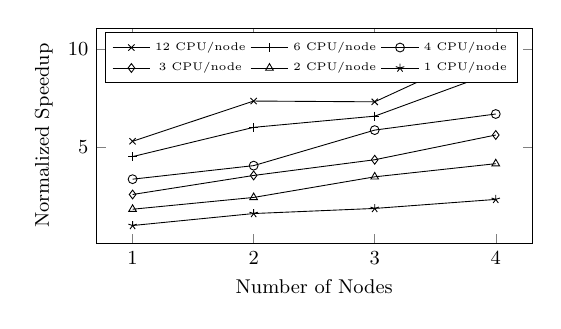
\begin{tikzpicture}[scale=0.8]
      \begin{axis}[
          xlabel=Number of Nodes,
          ylabel=Normalized Speedup,
          height=5cm,
          width=8.5cm,
          xtick={1,2,3,4},
          legend columns=3,
          font=\small
        ]
        \addplot coordinates {
% 12 CPUs
  (1, 5.29)
  (2, 7.34)
  (3, 7.30)
  (4, 10.14)
        };
        \addplot coordinates {
% 6 CPUs
  (1, 4.51)
  (2, 6.00)
  (3, 6.57)
  (4, 8.83)
        };
        \addplot coordinates {
% 4 CPUs
  (1, 3.36)
  (2, 4.05)
  (3, 5.86)
  (4, 6.68)
        };
        \addplot coordinates {
% 3 CPUs
  (1, 2.58)
  (2, 3.55)
  (3, 4.35)
  (4, 5.61)
        };
        \addplot coordinates {
% 2 CPUs
  (1, 1.83)
  (2, 2.43)
  (3, 3.48)
  (4, 4.15)
        };
        \addplot coordinates {
% 1 CPUs
  (1, 1.00)
  (2, 1.61)
  (3, 1.87)
  (4, 2.33)
        };
      \legend{12 CPU/node,6 CPU/node,4 CPU/node,3 CPU/node,2 CPU/node,1 CPU/node}
      \end{axis}
    \end{tikzpicture}
    \label{sfig:results2:perf}
  }

  \subtable[Execution Time Breakdown (all times in s)]{
    \scalebox{0.8}{
   \tiny
    \begin{tabular}{c@{\hspace{2pt}}cD{.}{.}{3}D{.}{.}{3}@{\hspace{2pt}}D{.}{.}{3}@{\hspace{2pt}}D{.}{.}{3}@{\hspace{2pt}}D{.}{.}{3}@{\hspace{2pt}}D{.}{.}{3}@{\hspace{2pt}}D{.}{.}{3}}
\toprule
GPUs/ & \# \\
node & nodes & \multicolumn{1}{c}{Wall Clock} & \multicolumn{1}{c}{Application} & \multicolumn{1}{c}{Copies} & \multicolumn{1}{c}{High-level} & \multicolumn{1}{c}{Low-level} & \multicolumn{1}{c}{Mapper} & \multicolumn{1}{c}{System} \\
\midrule
\multirow{4}{*}{$1$} & $1$ & 40.718 & 38.486 & 0.008 & 0.996 & 0.544 & 0 & 0\\
 & $2$ & 25.365 & 43.602 & 0.455 & 2.027 & 0.682 & 0 & 0.043\\
 & $3$ & 21.808 & 49.256 & 0.513 & 2.377 & 0.765 & 0 & 0.06\\
 & $4$ & 17.476 & 53.181 & 0.501 & 2.912 & 0.743 & 0 & 0.072\\
\midrule
\multirow{4}{*}{$2$} & $1$ & 22.289 & 38.55 & 0.009 & 1.694 & 0.68 & 0 & 0\\
 & $2$ & 16.787 & 51.081 & 0.573 & 2.373 & 0.756 & 0 & 0.056\\
 & $3$ & 11.706 & 49.502 & 0.733 & 2.661 & 0.749 & 0 & 0.072\\
 & $4$ & 9.817 & 50.798 & 0.86 & 2.755 & 0.735 & 0 & 0.1\\
\midrule
\multirow{4}{*}{$3$} & $1$ & 15.799 & 38.507 & 0.01 & 2.056 & 0.765 & 0 & 0\\
 & $2$ & 11.462 & 48.698 & 0.951 & 2.682 & 0.819 & 0 & 0.109\\
 & $3$ & 9.363 & 50.786 & 1.282 & 2.976 & 0.767 & 0 & 0.081\\
 & $4$ & 7.26 & 51.778 & 1.285 & 3.172 & 0.818 & 0 & 0.117\\
\midrule
\multirow{4}{*}{$4$} & $1$ & 12.11 & 39.296 & 0.011 & 2.17 & 0.827 & 0 & 0\\
 & $2$ & 10.05 & 49.799 & 1.145 & 3.023 & 0.82 & 0 & 0.24\\
 & $3$ & 6.951 & 51.216 & 1.367 & 3.137 & 0.798 & 0 & 0.12\\
 & $4$ & 6.093 & 52.183 & 1.216 & 3.317 & 0.782 & 0 & 0.135\\
\midrule
\multirow{4}{*}{$6$} & $1$ & 9.031 & 40.265 & 0.013 & 2.536 & 0.969 & 0 & 0\\
 & $2$ & 6.79 & 48.992 & 0.946 & 3.182 & 0.937 & 0 & 0.145\\
 & $3$ & 6.199 & 51.904 & 1.061 & 3.752 & 0.909 & 0 & 0.185\\
 & $4$ & 4.612 & 52.603 & 1.238 & 3.712 & 0.872 & 0 & 0.222\\
\midrule
\multirow{4}{*}{$12$} & $1$ & 7.704 & 45.959 & 0.03 & 4.01 & 1.765 & 0 & 0\\
 & $2$ & 5.547 & 65.432 & 1.019 & 4.762 & 1.328 & 0 & 0.232\\
 & $3$ & 5.577 & 68.74 & 1.059 & 5.922 & 1.384 & 0 & 0.322\\
 & $4$ & 4.017 & 67.662 & 1.19 & 4.882 & 1.22 & 0 & 1.485\\
\bottomrule \\
    \end{tabular}
}
    \label{sfig:results2:timers}
  }

  \caption{Fluid Results}
\end{figure}
